
\chapter{Evaluation}
\label{evaluation}

\section{Building an example model}
To confirm that the modelling system was adequate for the task, and to test the hypothesis laid out, the third required component of the project was constructed: an example model to be used to test the hypothesis. \par
\cref{fig:example_flows} shows how a workflow would begin to be developed using very simple Activity Diagrams as flows that are linking together. After all of the flows needed are broken down, any node on any flow that does not represent another flow (or the current flow itself, if the flow is recursive) would be an atom with activity that should be obvious by its name. \par
Two example models were built for the purposes of testing this hypothesis. They both modelled software development teams that adhered to some commonly used software development methodology. However, while one is a traditional Waterfall software development strategy as defined by the US Department of Defence in their original DOD-STD-2167A specification\cite{DEPARTAMENTOFDEFENSE1984}, the other is an Agile methodology, designed to fix many of the issues perceived to exist in the old Waterfall standard. Particularly, the Test Driven Development (TDD) methodology intends to fix the problem that exists when many bugs exist in a Waterfall system. The TDD method writes tests that nominally represent the functionality of a chunk of code, and subsequently write that code until the code passes the test, as can be seen in the full Activity Diagram for the TDD methodology in \cref{fig:agile_workflow}. \par

\begin{figure}[p]
    \centering
    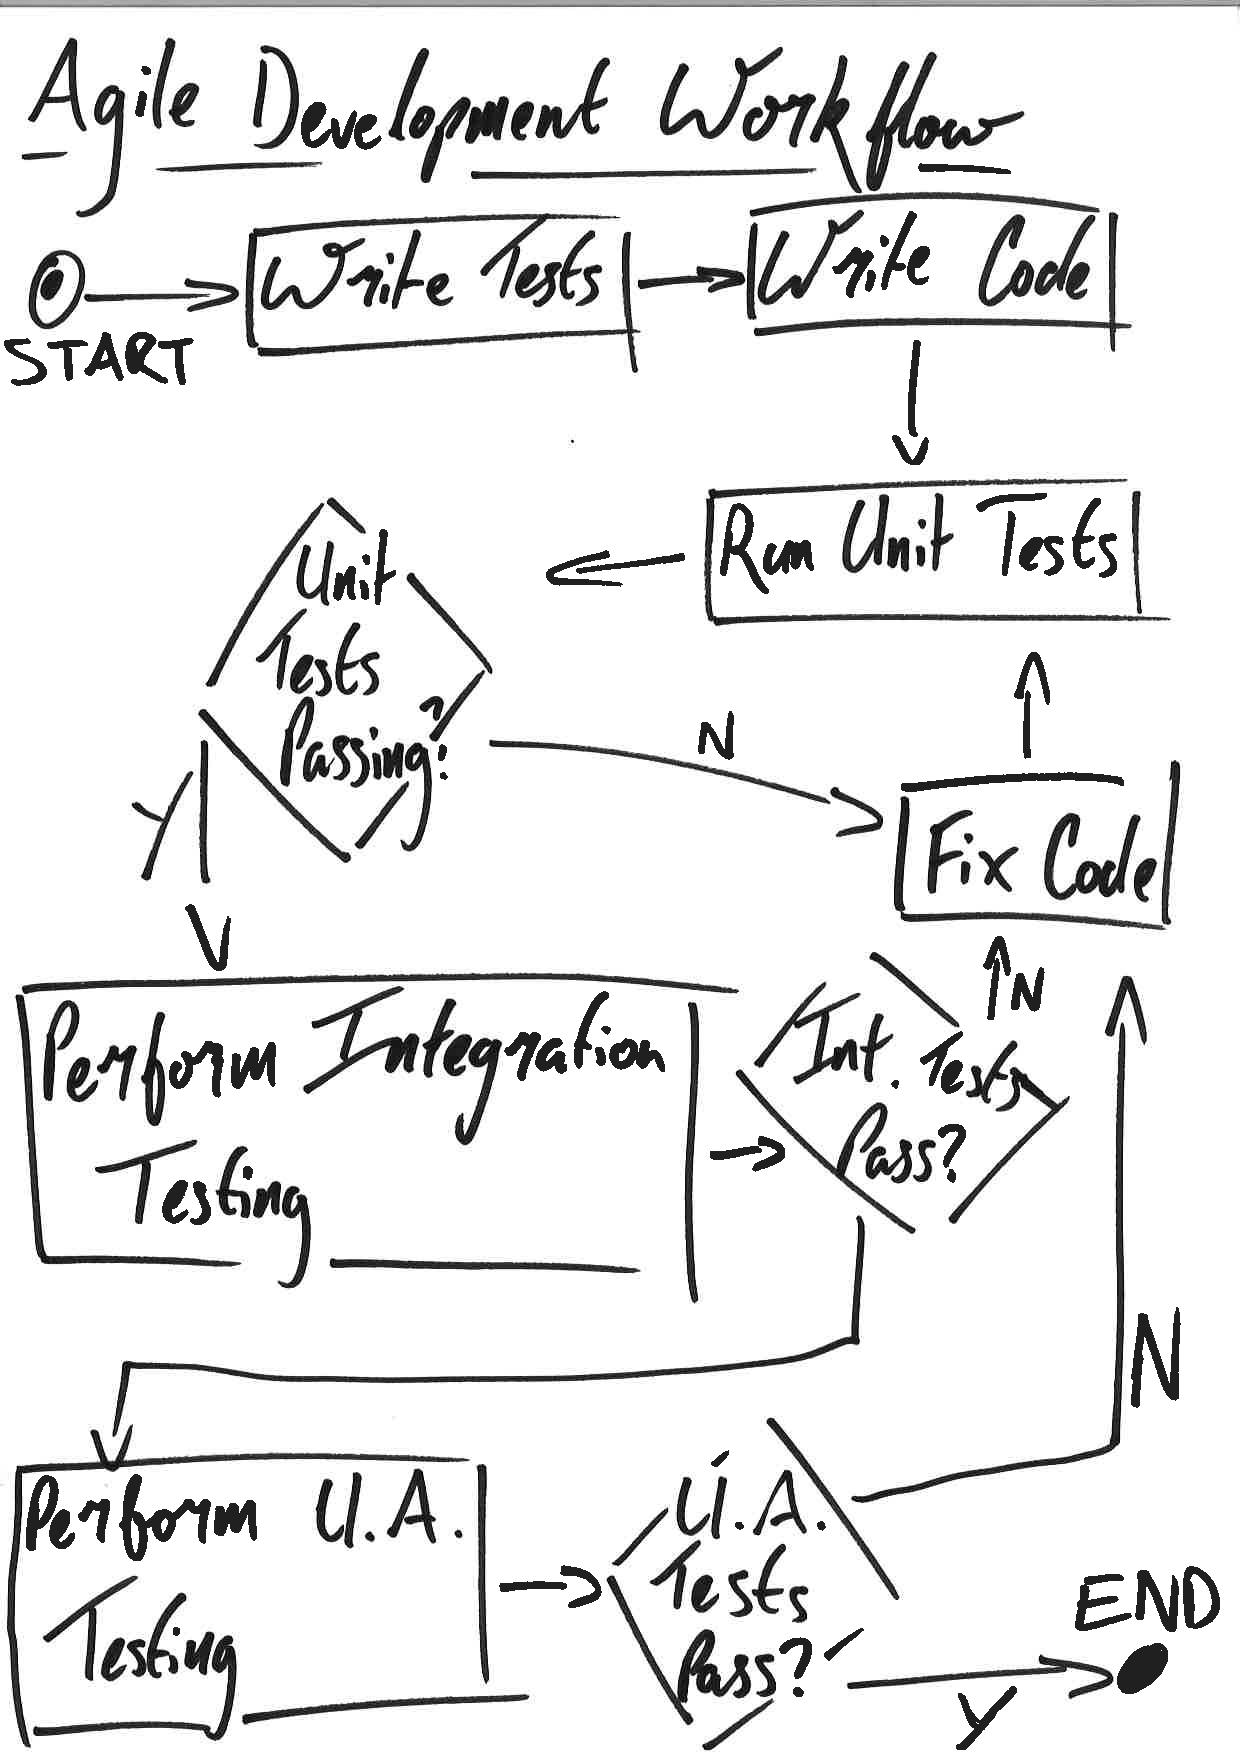
\includegraphics[width=0.9\textwidth]{images/Example_agile_flows.pdf}
    \caption{Some example Agile flows}
    \label{fig:example_flows}
\end{figure}

\begin{figure}[p]
    \centering
    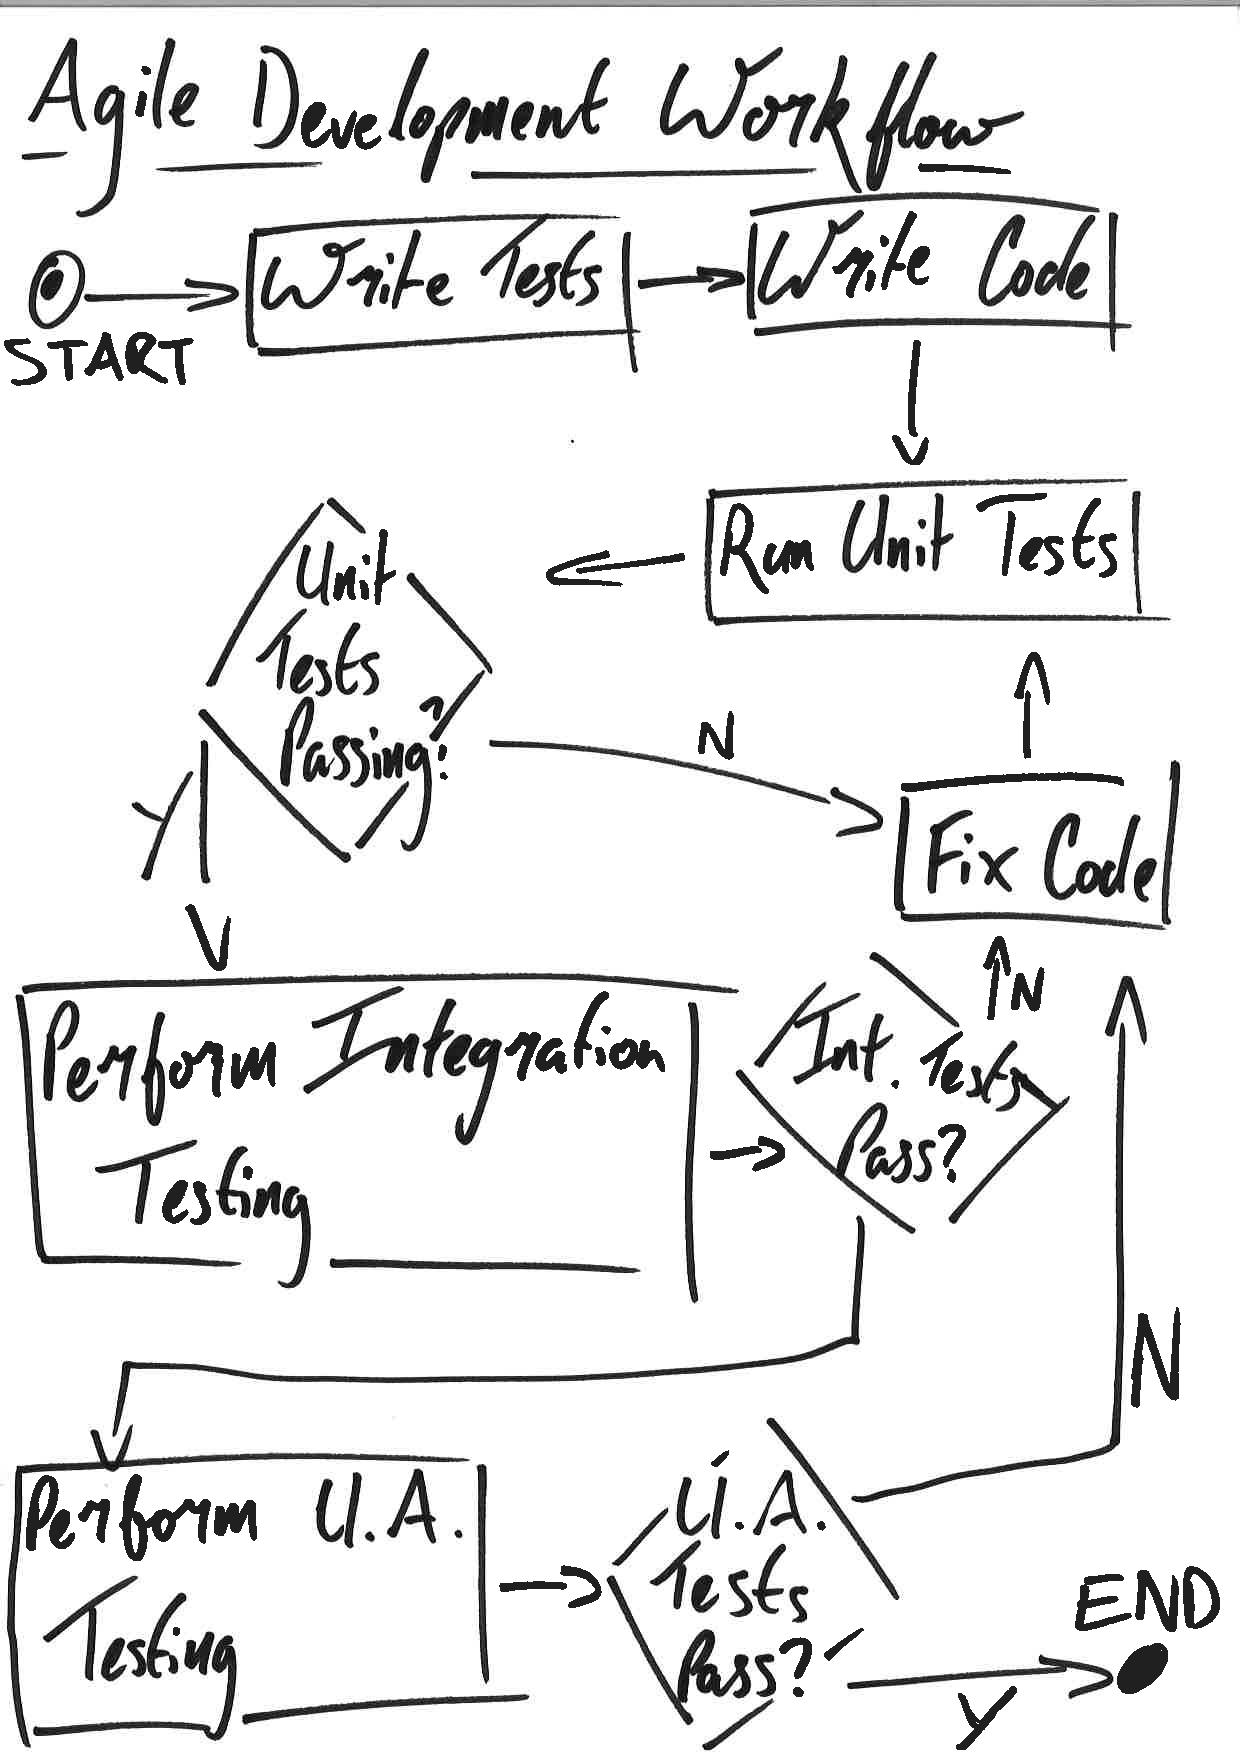
\includegraphics[width=0.9\textwidth]{images/Example_agile_flows.pdf}
    \caption{A full workflow for the development portion of a software product in Test-Driven Agile Development}
    \label{fig:agile_workflow}
\end{figure}

\subsection{Building flows}
Constructing the flows was as simple as following the understanding of the system from a high-level, not particularly detailed perspective, and drilling down on each individual node of the high-end view until more detail was extracted. In this way, the full TDD workflow that can be found in \cref{fig:agile_workflow} was built from the first flow which can be found at \cref{fig:example_flows}. This allowed very fast prototyping of the sociotechnical system in a manner which could be ported from the Activity Diagram to Python code very quickly. \par
As was noted in \cref{pictorial}, UML diagrams can be programmatically transformed into executable skeleton code with ease. In this way, converting the model to code ready for fuzzing would be even easier than it already is in the future. \par
This procedure was carried out for both the agile and waterfall workflows. 

\subsection{Building atoms}
Once flows were successfully built, all nodes on the Activity Diagrams that did not have a definition as another must be defined as atoms. Therefore, after the flows had been written as python programs, every function call that had no definition was indicated by the IDE, making the remaining work easy to spot. The errors in the flows were solved by creating the relevant atoms, together with the environment necessary to facilitate their effects, and the sociotechnical models were complete. \par
The sociotechnical environment was implemented as a Directed Acyclic Graph in the form of four different class definitions. Objects constructed from these classes were kept in a dictionary alongside some boolean flags and values which were used throughout the model, for modifying the program's behaviour and signalling things like tests passing to the rest of the model. \par

\subsection{Mutating the models}
Mutating the models was very easy. A fully mutated form of a code example from \cref{small_code_sample} was written like so:

\begin{pyglist}[language = python, encoding = utf8]
from base import mutate
import random

#Removes an action from a behaviour if the actor is stressed (50% chance)
def stressed(lines):
    if random.choice([True, False]):
        lines.remove(random.choice(lines))
    return lines
    

def implement_feature():
    make_new_feature()
    create_test_and_code()
    unit_test()
    integration_test()
    user_acceptance_test()

@mutate(stressed)
def unit_test():
    run_tests()
    while not environment.resources["unit tests passing"]:
        fix_recent_feature()
        run_tests()
\end{pyglist}\par
Mutating specific functions proved very easy with the system derived. The mutations could be directed to a specific workflow, was easy to write, and was also human-readable, particularly where it mattered in the flow definition.\par
Once concern was that, if a mutation function was convoluted or required complex logic to construct, it might be very easy to break the mutation library with a small bug. Another mutation function was then written to see whether anything complex would arise from deadlines being tight within a sociotechnical system:

\begin{pyglist}[language = python, encoding = utf8]
from base import mutate
import random

def cannot_meet_deadline(lines):
    if random.choice([True, False]):
        lines = lines[:random.randint(1, len(lines)-1)]
    return lines

@mutate(cannot_meet_deadline)
def unit_test():
    run_tests()
    while not environment.resources["unit tests passing"]:
        fix_recent_feature()
        run_tests()
\end{pyglist}\par
As can be seen, the additional mutation function was exactly as long and no more complex than the previous. Therefore, any simplification could satisfactorily be left for future work, as the mutation library implemented was adequate for the purposes of this project.\par

\section{Running a model}
Running a model was as simple as writing simple unit tests that call the highest-order function of the models created, because of the construction of the models according to the modelling system. \par
This is a result of the top-down approach to the sociotechnical model design. A side-effect of the full workflow being the first thing to be defined was that this first function can be run to run the whole sociotechnical system. An additional flow was added for testing purposes which implemented 50 features according to each methodology rather than just one, as this way the effects of the variance in the system would be more pronounced and therefore easier to detect. Naturally, this was very easy to implement, as it was simply a repetition of the main workflow.\par

\subsection{Carrying out experiments on the models}
The flows were run within a series of unit tests that confirmed that the sociotechnical environment was being affected in some way that made sense for the models that were constructed, with a flag to trigger mutations turned off. To confirm that the outcomes were not the results of the random seed at the time, the random seed was set as a variable in the sociotechnical environment.\par
Similar unit tests were then run with the environment turned off and turned on separately, so as to compare the effect of mutating each model. A method was implemented in each model to reset its sociotechnical environment to some base state, which meant that a model could be run indefinitely many times in the same unit test. \par
Once the mutation library was verified to be working, a unit test was constructed that ran each model twice --- once mutated, and once in its unmodified state --- and calculated the difference in the time each model took to implement 50 features when put under stress in its unit testing phase. The difference was then compared between the two executions of the models. \par
If the delta in time taken was less for the agile model than it was for the waterfall model, it would be confirmed that influencing the models using code fuzzing was having the intended effect, as an agile flow should operate better than a waterfall method when put under sociotechnical stress. The unit test was thus written so that it would pass if this was true, indicating that the experiment's hypothesis was validated. \par
When the test was run, it passed, validating the experiment. \par


\section{Evaluating the tools used}

